\section{Real-Hardware Fine-Tuning}
\label{appendix:finetuning}

\subsection{Motivation}

Despite domain randomization and sensor modeling reducing the
sim-to-real settling-time gap to $3.0\times$
(Appendix~\ref{appendix:sim2real}), the question remains whether
online fine-tuning on real hardware can further close this gap.
We fine-tune three deployed policies on real hardware: the two best
sim-trained agents, one on-policy (PPO~(BZ+DR)) and one off-policy (TD3),
and the world-model policy PPO~(WM), to compare adaptation strategies.

\subsection{Protocol}

We fine-tune all three policies directly on the real system in the
\texttt{BalancerReal} Gym environment, with an
augmented reward signal:
\begin{equation}
  r_t^{\text{FT}} = \mathrm{clip}\bigl(r_t^{\text{balanced}} + d_t,\; -1,\; 1\bigr)
\end{equation}
where $d_t \in \{0, 1\}$ is the binary infrared dip-sensor signal
(1 while the ball physically obstructs the beam at the arc's lowest
point, 0 otherwise). The beam is broken over an active band narrower
than the ball diameter, so $d_t$ fires only within a few millimeters of
true center; this is the raw hardware bit, not the wider offline angular
proxy ($\theta_\text{center} = 0.007$\,rad) that
Appendix~\ref{appendix:dataset_details} uses when rebuilding the logged
dataset. It provides a strong, noise-free reward signal at the exact
balancing target that is unavailable in simulation.
The environment does not terminate on cart or ball limits; only the 30\,s
\texttt{TimeLimit} truncates an episode, and the per-step reward is the
clipped balanced-plus-dip signal above, not overwritten at the limit.

Table~\ref{tab:ft_protocol} lists the fine-tuning hyperparameters.
All three policies use a reduced learning rate ($10^{-4}$, vs.\ $3\times10^{-4}$
for PPO and $10^{-3}$ for TD3 during sim training) to prevent
catastrophic forgetting.

\begin{table}[!t]
\centering
\renewcommand{\arraystretch}{1.15}
\caption{Fine-tuning protocol. The PPO~(BZ+DR) base model is the S-curve
  development policy (98\% hardware SR); Table~II (main paper) reports the
  matched first-order-lag checkpoint at 96\% (Appendix~\ref{appendix:rl_fairness}).}
\label{tab:ft_protocol}
\begin{tabular}{lcc}
\toprule
\textbf{Parameter} & \textbf{PPO FT} & \textbf{TD3 FT} \\
\midrule
Base model           & PPO (BZ+DR)           & TD3 (DR)              \\
Learning rate        & $10^{-4}$             & $10^{-4}$             \\
Total steps          & 50\,000               & 50\,000               \\
Wall-clock time      & $\sim$50\,min         & $\sim$50\,min         \\
Episodes             & $\sim$83              & $\sim$83              \\
Checkpoint freq      & 5\,000 steps          & 5\,000 steps          \\
Reward               & balanced + IR dip     & balanced + IR dip     \\
Entropy coeff        & 0.005                 & --                   \\
\bottomrule
\end{tabular}
\end{table}

\subsection{Results}

Table~\ref{tab:ft_results} compares pre-FT and post-FT hardware
performance, and Fig.~\ref{fig:finetuning_results} shows it graphically: the
PPO~(WM) settling-time distributions before and after fine-tuning differ
modestly (both 100\% SR), alongside the success-rate comparison
for all three fine-tuned models.

\begin{table}[!t]
\centering
\renewcommand{\arraystretch}{1.15}
\caption{Fine-tuning results: hardware evaluation.
         PPO~(WM) evaluated on 50 stratified trials;
         PPO~(BZ+DR) and TD3 on 10 trials each.}
\label{tab:ft_results}
\begin{tabular}{lccccc}
\toprule
\textbf{Model} & \textbf{N} & \textbf{SR} & \textbf{Mean (s)}
  & \textbf{Med (s)} & \textbf{Max (s)} \\
\midrule
\multicolumn{6}{l}{\textit{Pre-fine-tuning:}} \\
PPO (WM)           & 50  & 100\% & 6.84 & 3.64 & --  \\
PPO (BZ+DR)        & 10  & 100\% & 4.98 & --  & 13.66 \\
TD3 (DR)           & 10  & 100\% & 8.16 & --  & 23.00 \\
\midrule
\multicolumn{6}{l}{\textit{Post-fine-tuning:}} \\
PPO (WM) + FT      & 50  & 100\% & 7.03 & 5.41 & --  \\
PPO (BZ+DR) + FT   & 10  &  90\% & 6.50 & 4.66 & 21.71 \\
TD3 (DR) + FT      & 10  &  80\% & 8.60 & 5.85 & 26.65 \\
\bottomrule
\end{tabular}
\end{table}

\begin{figure}[!t]
  \centering
  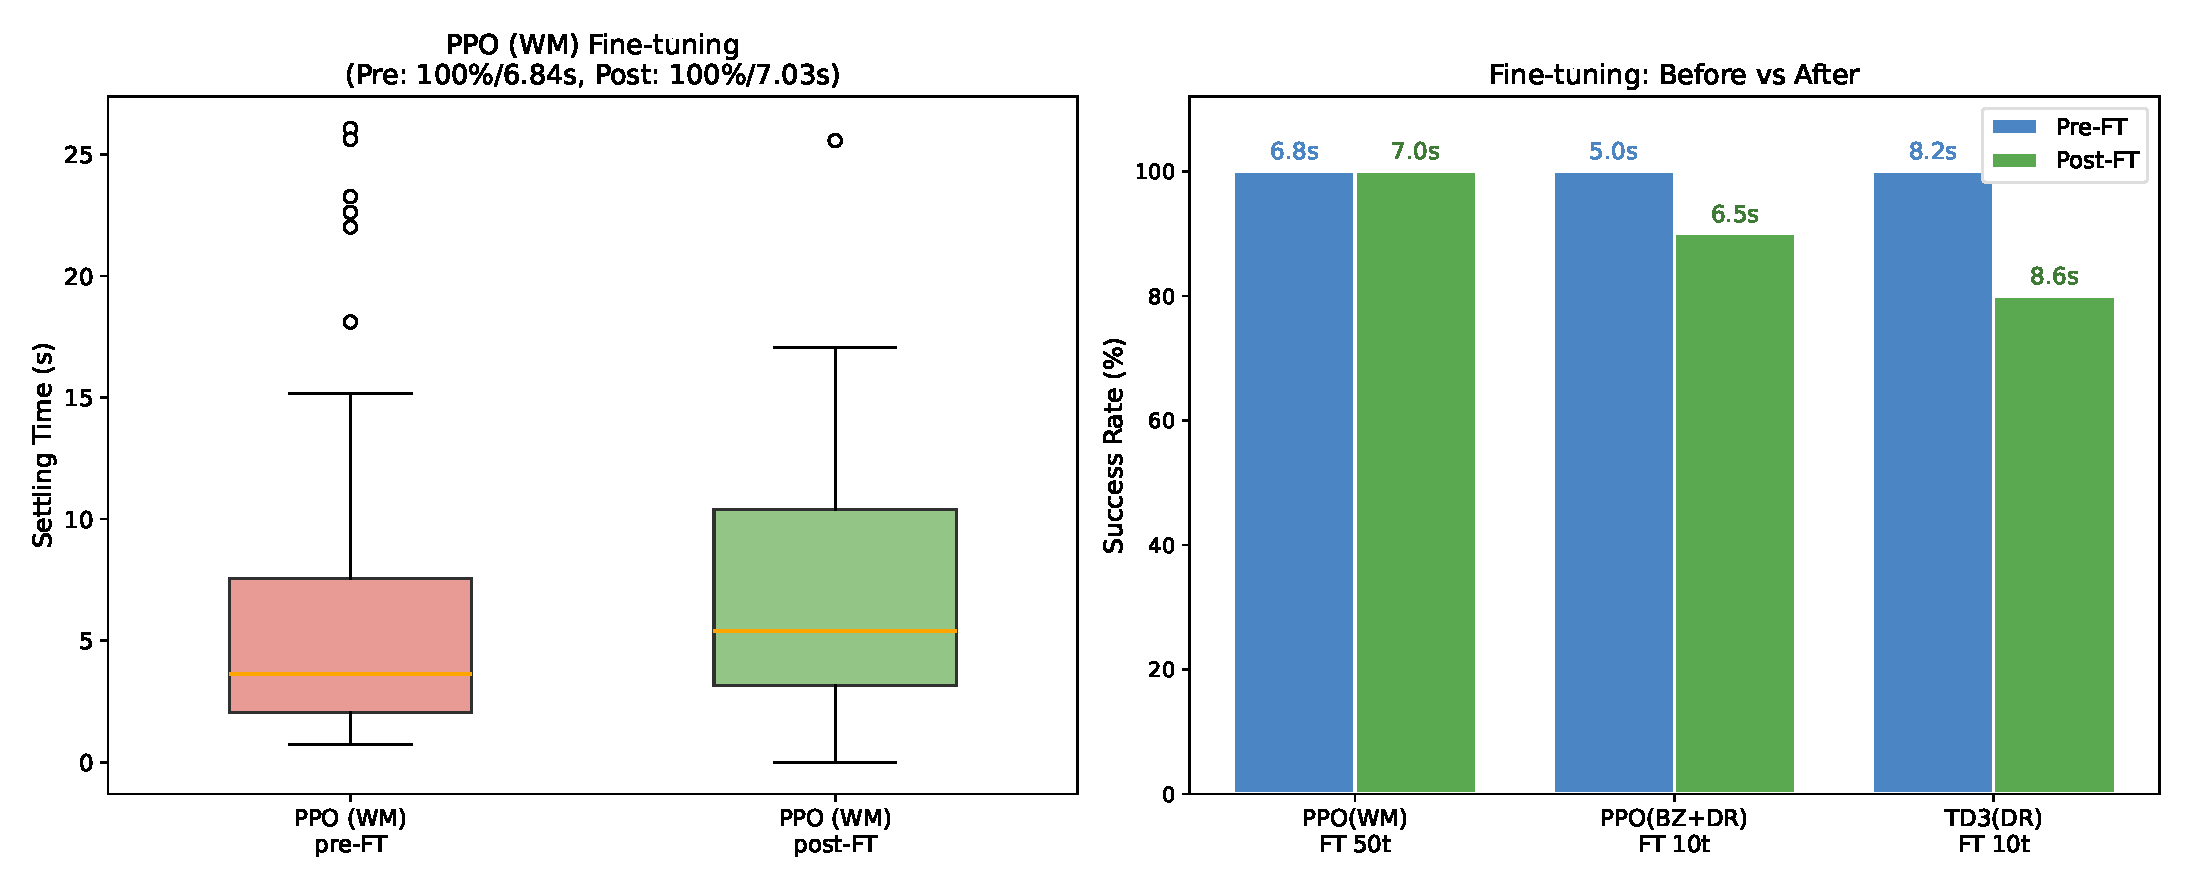
\includegraphics[width=\columnwidth]{figures/finetuning_results.eps}
  \caption{Fine-tuning comparison. Left: PPO~(WM) settling time
    distribution before and after fine-tuning (50 trials each, both 100\% SR).
    Right: success rate comparison for all fine-tuned models with
    mean settling time annotations.}
  \label{fig:finetuning_results}
\end{figure}

\subsection{Analysis}

\paragraph{PPO~(WM) fine-tuning.}
The world-model PPO, fine-tuned for 50K steps on real hardware,
retains 100\% SR, and the before/after settling-time distributions differ
in shape (a higher post-fine-tuning median, 3.64\,s~$\to$~5.41\,s, and a
heavier upper tail), but not significantly (Mann-Whitney on settling
times, $p = 0.27$); the means stay close (6.84\,s~$\to$~7.03\,s).
The mean episode reward dips at the onset of fine-tuning and then recovers
slowly over the 50K steps, ending near its starting level, so the fine-tuning
step itself is not failing; the policy changes only modestly under real-data
gradients on this budget. On this 50-trial evaluation, online adaptation did
not produce a measurable improvement, consistent with the world-model policy
already capturing much of the relevant dynamics.

\paragraph{Sim-trained model fine-tuning.}
On a matched 10-trial hardware evaluation, fine-tuning did not improve either
policy and moved each by one or two of ten trials: PPO~(BZ+DR) from 10/10 to
9/10 and TD3 from 10/10 to 8/10, both with slightly longer settling. These 10-trial
figures sit against the 50-trial baselines of 98\% (PPO~(BZ+DR))
and 92\% (TD3), so the effect is small in absolute terms; at 10 trials these
one- and two-trial changes are within sampling noise, and we observe no
improvement from fine-tuning on either paradigm at this budget.

\paragraph{Root causes.}
Three factors plausibly contribute. The first is simply too little data: 50k
steps is roughly 83 episodes per policy (30\,s trials at 20\,Hz), against the
3M (PPO) and 1M (TD3) steps of the original simulation training, far too little
real experience to learn a meaningful improvement. The second is catastrophic
forgetting: even at the reduced learning rate ($10^{-4}$), gradient updates
from a handful of real episodes partly overwrite the simulation-trained
policy, and the low-reward episodes from at-wall starts corrupt the value
function. The third is that the pre-fine-tuning models are already near their
ceiling: PPO~(BZ+DR) reaches 98\% over 50 hardware trials without any
fine-tuning, and its single failure, on a center start, may need an
architectural change rather than more data to close.

\paragraph{On-policy vs.\ off-policy.}
PPO changed by one of ten trials and TD3 by two; at this sample size the
difference between them is not meaningful, and neither improved with this
budget.

\paragraph{Implications.}
These results validate the sim-to-real approach taken in this work:
careful simulation modeling produces policies that transfer effectively
without online adaptation, and PPO~(BZ+DR) already sits near the
reliability ceiling on hardware. On this budget online fine-tuning does
not help: as the reward curve shows, the policy first unlearns and then
relearns, spending the real interaction returning to where it started
rather than improving. Because the deployed policy is already
near-ceiling and a learned world model already captures the system's
dynamics well (its prediction accuracy plateaus by roughly 100k
transitions, Appendix~\ref{appendix:world_model}), training PPO inside
that world model (PPO-WM) or relying on one-shot transfer is a more
effective use of effort than online fine-tuning on the physical rig.

Future work could investigate:
\begin{itemize}
  \item Longer fine-tuning budgets ($>$500K real steps,
    $\sim$8 hours of continuous operation).
  \item Replay buffer seeding with sim data (for TD3/SAC)
    to prevent catastrophic forgetting.
  \item Residual policy learning: training a small correction
    network on top of the frozen sim policy.
  \item System identification: using real trajectories to
    update the simulation model rather than the policy directly.
\end{itemize}
